\documentclass[11pt]{article}
\usepackage[margin=0.88in]{geometry}
\usepackage{mathptmx}
\usepackage[T1]{fontenc}
\usepackage{amsmath}
\usepackage{booktabs}
\usepackage{graphicx}
\usepackage{array}
\usepackage{enumitem}
\usepackage{caption}
\usepackage{url}
\usepackage{tikz}
\usetikzlibrary{shapes.geometric, arrows.meta, positioning, calc}

% --------------------------------------------------------------------------------------------
% Custom formatting commands
\newcommand{\topicTitle}[1]{
    \vspace{0.35em}\noindent{\fontsize{11}{13.2}\selectfont \textbf{#1}}\par\vspace{0.2em}
}

\newcommand{\qLabel}[1]{
    {\fontsize{10.2}{12.2}\selectfont \textbf{#1}}
}
% --------------------------------------------------------------------------------------------

\begin{document}

% ============================================================================================
% PAGE 1: TITLE PAGE
% ============================================================================================
\begin{center}
    
\includegraphics[width=0.28\textwidth]{vnit-logo.jpg}\\[1.0cm]
    
    {\large \textbf{Group Members}}\\[0.25cm]
    \begin{tabular}{l c l}
        Student 1: Gaurav Acharya & --- & [MT26MCS024] \\
        Student 2: Sandeep & --- & [MT26MCS032]
    \end{tabular}
    
    \vspace{0.8cm}
    
    {\large \textbf{Guide Name}}\\[0.25cm]
    Dr. A. S. Mokhade
    
    \vspace{0.8cm}
    
    {\large \textbf{Practical Title:}}\\[0.25cm]
    CSP529: Technical Writing \& Publishing\\[0.15cm]
    Practical 10: From Research Gap to a Defensible Research Proposal\\[0.15cm]

    \vspace{0.8cm}
    
    {\large \textbf{Problem Statement}}\\[0.2cm]
    Transforming a Refined Research Question into a Defensible Research Proposal: \\
    Research Objectives, Testable Hypotheses, and Evaluation Framework.
    

\end{center}
\noindent


% ============================================================================================
% PAGE 2: STAGE 1 (TASK A1, TASK A2)
% ============================================================================================
\newpage
{\centering\fontsize{13}{16}\selectfont\textbf{Stage 1 --- Revisit the Research Question and Gap}\par}
\vspace{0.3em}

\topicTitle{Task A: Research Question and Gap Specification}

In Practicals~7 and 8, our group examined whether Shortest Remaining Time First (SRTF) truly maintains its theoretical superiority over non-preemptive First-Come-First-Served (FCFS) in real systems [1, 2]. While textbook proofs show SRTF minimizes average waiting time, our literature search in Practical~8 revealed a critical limitation in published studies: existing proofs of SRTF's noise resilience (e.g., Lu et al.~[3] and Wierman \& Nuyens~[4]) rely on costless preemption ($t_{cs} = 0$) and heavily skewed Pareto workloads. Below, we trace our refined research question, articulate the specific gap, examine the closest literature, and explain why our study remains necessary.

\begin{itemize}[leftmargin=1.2em, itemsep=0.45em, parsep=0pt]

    \item \qLabel{1. Final Research Question Developed in Practical 8:} \\
    Following our adversarial literature search in Practical~8 (Stage~5), we refined our provisional question to isolate non-skewed workloads and realistic hardware context switching:
    \begin{itemize}[label=$\circ$, leftmargin=1.2em, itemsep=0.2em]
        \item \textbf{Provisional Question (Practical 7):} \textit{Under what burst prediction error thresholds and context-switch latencies does SRTF fail to outperform non-preemptive FCFS in average waiting time?}
        \item \textbf{Evolutionary Critique (Practical 8 Search Insights):} Adversarial analysis revealed that size-based scheduling is exceptionally resilient to noise when workloads possess heavy tails ($C_v \gg 1$), because coarse job sizing successfully prevents giant jobs from creating catastrophic convoys. Thus, examining prediction noise alone was scientifically insufficient; we had to explicitly isolate workloads where workload variance does not mask preemption costs.
        \item \textbf{Final Refined Question (Practical 8):} \textit{``Under what combination of burst prediction error ($\epsilon$) and hardware context-switch latency ($t_{cs}$) does Shortest Remaining Time First (SRTF) cease to outperform non-preemptive First-Come-First-Served (FCFS) in average waiting time, specifically across non-heavy-tailed (uniform and exponential) CPU-burst workload distributions?''}
    \end{itemize}

    \vspace{0.3em}
    \item \qLabel{2. Specific Research Gap:} \\[0.15em]
    \noindent\fbox{%
    \parbox{\dimexpr\linewidth-2\fboxsep-2\fboxrule\relax}{%
    \vspace{0.2em}
    Classical scheduling theory establishes Shortest Remaining Time First (SRTF) as optimal for minimizing average waiting time in uniprocessor queues. However, this optimality fundamentally assumes perfect advance knowledge of burst durations ($\epsilon = 0$) and zero context-switch latency ($t_{cs} = 0$). Although published studies show that size-based scheduling resists estimation noise alone in heavy-tailed workloads, they uniformly assume costless, instantaneous preemption. In physical operating systems, burst prediction errors cause frequent erroneous preemptions, incurring dispatcher overheads and severe CPU cache and TLB invalidation penalties. The unaddressed research gap is the empirical and analytical quantification of the multi-variable crossover boundary $(\epsilon, t_{cs})$ where SRTF's latency advantage over non-preemptive First-Come-First-Served (FCFS) degrades or reverses ($AWT_{\text{SRTF}} \ge AWT_{\text{FCFS}}$) in non-heavy-tailed workloads (e.g., uniform and exponential distributions), where preemption costs cannot be masked by workload skew.
    \vspace{0.2em}%
    }%
    }


\end{itemize}

% ============================================================================================
% PAGE 3: STAGE 1 (TASK A3, TASK A4)
% ============================================================================================
\newpage
\begin{itemize}[leftmargin=1.2em, itemsep=0.45em, parsep=0pt]

    \item \qLabel{3. Two Published Studies Most Closely Related to the Question:}
    \begin{enumerate}[label=(\alph*), leftmargin=1.2em, itemsep=0.35em, parsep=0pt]
        \item \textbf{Lu, Sheng, and Dinda (2004) [3] --- \textit{``Size-based scheduling policies with inaccurate scheduling information''}:} \\
        Evaluating web and supercomputing traces, the authors demonstrated that size-based scheduling (SRPT) is surprisingly robust to estimation error, beating FCFS even when correlation dropped to $r \approx 0.5$ because coarse sorting still prevents huge jobs from creating convoys. 
        
        \textit{Critical Limitation and Inapplicability to our Gap:} However, Lu et al.\ assumed instantaneous preemption ($t_{cs} = 0$) and evaluated only heavy-tailed Pareto distributions. Their simulations ignored hardware dispatcher latency, CPU register switching, and cache-reload degradation, leaving real hardware switching penalties and non-skewed burst profiles completely unaddressed.

        \item \textbf{Wierman and Nuyens (2008) [4] --- \textit{``Scheduling despite inexact job-size information''}:} \\
        Wierman and Nuyens developed the analytical $\epsilon$-SMART framework for $M/G/1$ queues, proving mathematically that under bounded multiplicative prediction noise, mean response time degrades smoothly by at most $(1+\epsilon)^2$ in heavy-tailed traffic.
        
        \textit{Critical Limitation and Inapplicability to our Gap:} While mathematically rigorous, their proofs explicitly rely on costless preemption and focus on asymptotic heavy-tailed regimes. They did not model non-zero context-switch penalties ($t_{cs} > 0$), cache reload overheads ($t_{cache} > 0$), or low-variance burst distributions ($C_v \le 1$), where erroneous preemptions rapidly destroy queuing advantages.
    \end{enumerate}

    \vspace{0.3em}
    \item \qLabel{4. Defensible Justification of the Proposed Research:} \\
    Our proposed investigation remains necessary and defensible for three fundamental reasons:
    \begin{enumerate}[label=(\roman*), leftmargin=1.2em, itemsep=0.3em, parsep=0pt]
        \item \textbf{Invalidation of Costless Preemption in Modern Hardware:} On modern deep-pipelined, hierarchical-memory CPUs, a context switch incurs far more than the simple dispatcher instruction sequence ($t_{cs} \approx 2$--$5\,\mu\text{s}$). Cold-cache and TLB misses ($t_{cache}$) add tens of microseconds of stall time [5]. Under estimation noise, SRTF triggers ``erroneous preemptions''---suspending a job for one that is actually longer. When preemption incurs physical memory penalties, its cumulative cost can quickly outstrip SRTF's marginal queuing benefit.
        \item \textbf{Absence of Workload Skew Protection:} In heavy-tailed Pareto workloads (e.g., Web traffic), 1\% of jobs consume 99\% of CPU cycles. Preventing convoys behind these giant jobs yields massive waiting-time savings that easily dwarf switching costs. However, in non-heavy-tailed workloads (exponential and uniform, $C_v \le 1$) typical of transactional microservices and numeric pipelines, burst lengths are relatively uniform. SRTF's anti-convoy gains shrink dramatically, exposing the scheduling policy to net throughput degradation from preemption thrashing.
        \item \textbf{Bridging Mathematical Theory and Systems Reality:} Classical proofs establish theoretical optimality, while empirical OS benchmarks exhibit unpredictable kernel noise. Our study bridges this divide by mapping the precise parametric frontier $(\epsilon^*, t_{cs}^*)$ where algorithmic inversion occurs, establishing actionable thresholds for OS engineers.
    \end{enumerate}

\end{itemize}

% ============================================================================================
% PAGE 4: STAGE 1 (DELIVERABLE 1 & THEORETICAL QUEUEING CONTEXT)
% ============================================================================================
\newpage
\topicTitle{Deliverable 1: Consolidated Research Gap Statement and Supporting Citations}

Below, we synthesize our refined research question, core gap, published literature limitations, and defensible justification into a consolidated reference summary.

\vspace{0.2em}
\noindent\fbox{%
\parbox{\dimexpr\linewidth-2\fboxsep-2\fboxrule\relax}{%
\vspace{0.25em}
\textbf{1. Final Research Question:} \\
\textit{``Under what combination of burst prediction error ($\epsilon$) and hardware context-switch latency ($t_{cs}$) does Shortest Remaining Time First (SRTF) cease to outperform non-preemptive First-Come-First-Served (FCFS) in average waiting time, specifically across non-heavy-tailed (uniform and exponential) CPU-burst workload distributions?''} \\[0.3em]
\textbf{2. Core Research Gap Statement :} \\
Classical scheduling theory establishes SRTF as optimal for minimizing average waiting time in uniprocessor queues. However, this optimality fundamentally assumes perfect advance knowledge of burst durations ($\epsilon = 0$) and zero context-switch latency ($t_{cs} = 0$). Although published studies show that size-based scheduling resists estimation noise alone in heavy-tailed workloads, they uniformly assume costless, instantaneous preemption. In physical operating systems, burst prediction errors cause frequent erroneous preemptions, incurring dispatcher overheads and severe CPU cache and TLB invalidation penalties. The unaddressed research gap is the empirical and analytical quantification of the multi-variable crossover boundary $(\epsilon, t_{cs})$ where SRTF's latency advantage over non-preemptive FCFS degrades or reverses ($AWT_{\text{SRTF}} \ge AWT_{\text{FCFS}}$) in non-heavy-tailed workloads (e.g., uniform and exponential distributions), where preemption costs cannot be masked by workload skew. \\[0.3em]
\textbf{3. Closely Related Literature \& Key Limitations:}
\begin{itemize}[label=$\bullet$, leftmargin=1.2em, itemsep=0.15em]
    \item \textbf{Lu, Sheng, and Dinda (2004) [3]:} Proved SRPT noise tolerance in Web server traces ($r \approx 0.5$); strictly assumed $t_{cs} = 0$ and heavy-tailed Pareto distributions.
    \item \textbf{Wierman and Nuyens (2008) [4]:} Derived $\epsilon$-SMART analytical degradation bounds; strictly assumed zero preemption cost and heavy-tailed traffic.
\end{itemize}
\textbf{4. Novelty and Practical Necessity:} \\
Quantifies the exact multi-variable threshold contour $(\epsilon^*, t_{cs}^*)$ where real hardware switching penalties and low workload skew cause non-preemptive FCFS to outperform SRTF, guiding adaptive OS scheduler design.
\vspace{0.25em}%
}%
}

\vspace{0.4em}
\topicTitle{Theoretical Queueing Foundations Underlying the Research Gap}

To ground our research question mathematically, consider an $M/G/1$ queue with Poisson arrivals at rate $\lambda$, mean burst duration $E[X]$, and service variance $\text{Var}(X)$. The Pollaczek-Khinchine formula defines mean waiting time under non-preemptive FCFS [6]:
\begin{equation}
W_{\text{FCFS}} = \frac{\lambda E[X^2]}{2(1-\rho)} = \frac{\lambda E[X]^2 (1 + C_v^2)}{2(1-\rho)}
\end{equation}
where $C_v = \frac{\sqrt{\text{Var}(X)}}{E[X]}$ is the coefficient of variation, and $\rho = \lambda E[X]$ is traffic load. When $C_v \gg 1$ (heavy-tailed), $W_{\text{FCFS}}$ diverges rapidly due to giant jobs monopolizing the CPU. Under SRTF with zero context-switch latency ($t_{cs} = 0$), prioritization bounds the delay of short tasks, keeping $W_{\text{SRTF}} \ll W_{\text{FCFS}}$ even when estimates are noisy [4]. 

However, in non-heavy-tailed workloads ($C_v \le 1$), $W_{\text{FCFS}}$ remains inherently well-behaved. If preemptive scheduling is introduced with estimation error $\epsilon$, every erroneous preemption injects non-productive dispatcher latency $t_{cs}$ and cache invalidation delay $t_{cache}$. The effective service demand inflates to $X_{\text{eff}} = X + \sum (t_{cs} + t_{cache})$. When $C_v$ is low, the anti-convoy queuing benefit of size-based ordering is minimal ($\Delta W_{\text{ideal}} \approx 10$--$20\%$), allowing preemption latency inflation to rapidly invert the inequality such that $AWT_{\text{SRTF}} \ge AWT_{\text{FCFS}}$.

% ============================================================================================
% PAGE 5: STAGE 2 (TASK B, TASK C)
% ============================================================================================
\newpage
{\centering\fontsize{13}{16}\selectfont\textbf{Stage 2 --- Define Research Objectives and Hypotheses}\par}
\vspace{0.3em}

\topicTitle{Task B: Research Objectives}

We define three clear, measurable research objectives to evaluate the identified crossover boundary:
\begin{itemize}[leftmargin=1.2em, itemsep=0.35em, parsep=0pt]

    \item \qLabel{Objective 1 ($O_1$): Quantification of Preemption and Cache Overhead under Estimation Noise} \\
    Quantify the empirical frequency of erroneous preemptions and resulting CPU time lost to context-switch latency ($t_{cs} \in [1, 50]\,\mu\text{s}$) and L1/L2 cache-reload delays ($t_{cache} \in [0, 20]\,\mu\text{s}$) across uniform and exponential CPU-burst distributions under synthetic prediction errors $\epsilon \in [0\%, 100\%]$. This evaluates how estimation noise scales dispatcher state-saving and cold-cache stalls relative to useful execution time.

    \item \qLabel{Objective 2 ($O_2$): Mapping the Multi-Variable Crossover Boundary $(\epsilon^*, t_{cs}^*)$} \\
    Empirically map and model the multi-variable crossover boundary $(\epsilon^*, t_{cs}^*)$ where SRTF's average waiting time degrades to equal or exceed that of non-preemptive FCFS ($AWT_{\text{SRTF}} \ge AWT_{\text{FCFS}}$) across normalized CPU loads $\rho \in \{0.3, 0.5, 0.7, 0.9\}$. This isolates the exact parametric frontier dividing SRTF-superior and FCFS-superior regimes under varying queue congestion.

    \item \qLabel{Objective 3 ($O_3$): Workload Skew Sensitivity and Evaluation of an Adaptive Fallback Policy} \\
    Evaluate how workload variance ($C_v \in [0.58, 4.0]$) shifts this crossover boundary, comparing non-heavy-tailed distributions against heavy-tailed Pareto workloads. Furthermore, design and benchmark a threshold-triggered heuristic that dynamically falls back to non-preemptive FCFS when measured runtime estimation error and switching overhead exceed the identified crossover contour.

\end{itemize}

\vspace{0.35em}
\topicTitle{Task C: Research Hypotheses}

We formulate two testable hypotheses directly addressing these performance trade-offs:

\begin{itemize}[leftmargin=1.2em, itemsep=0.35em, parsep=0pt]

    \item \qLabel{Hypothesis 1 ($H_1$): Algorithmic Inversion under Realistic Overheads in Low-Variance Workloads} \\
    \textbf{Proposition:} In non-heavy-tailed CPU workloads (exponential and uniform distributions with $C_v \le 1$), there exists a critical prediction error threshold $\epsilon^* < 30\%$ and realistic context-switch latency $t_{cs}^* \le 15\,\mu\text{s}$ at which non-preemptive FCFS achieves lower average waiting time than SRTF ($AWT_{\text{FCFS}} < AWT_{\text{SRTF}}$). \\
    \textbf{Theoretical Rationale:} When burst lengths have low variance ($C_v \le 1$), jobs are relatively uniform, so size-based ordering offers minimal anti-convoy gains. When prediction noise triggers false preemptions, cumulative switching and cold-cache stalls quickly exceed SRTF's marginal queuing benefit, making arrival-ordered execution faster. \\
    \textbf{Evidence Criteria:} \textit{Supported} if discrete-event simulations show $AWT_{\text{SRTF}} > AWT_{\text{FCFS}}$ at $\epsilon \ge 25\%$ and $t_{cs} = 10\,\mu\text{s}$ under exponential arrivals; \textit{contradicted} if SRTF maintains lower average waiting times across all realistic error ($\epsilon \le 50\%$) and latency ($t_{cs} \le 50\,\mu\text{s}$) ranges.

    \item \qLabel{Hypothesis 2 ($H_2$): Workload-Variance Dependence of the Preemption Crossover Boundary} \\
    \textbf{Proposition:} The crossover boundary $(\epsilon^*, t_{cs}^*)$ is positively correlated with the coefficient of variation ($C_v$) of the burst distribution; specifically, transitioning from heavy-tailed ($C_v \gg 1$) to low-variance ($C_v \le 1$) workloads contracts SRTF's dominance area in the $(\epsilon, t_{cs})$ plane by at least $50\%$. \\
    \textbf{Theoretical Rationale:} Heavy-tailed workloads (e.g., Pareto) have extreme service skews where preventing convoys behind giant jobs yields large waiting-time reductions that absorb substantial switching delays. In low-variance workloads, this protective buffer is absent, dramatically lowering the preemption cost SRTF can tolerate. \\
    \textbf{Evidence Criteria:} \textit{Supported} if phase diagrams show Pareto workloads sustain SRTF dominance up to $\epsilon^* > 65\%, t_{cs}^* > 75\,\mu\text{s}$ while uniform workloads collapse at $\epsilon^* \le 20\%, t_{cs}^* \le 10\,\mu\text{s}$ ($>50\%$ dominance area contraction); \textit{contradicted} if the boundary remains within $\pm 10\%$ across distributions.

\end{itemize}

% ============================================================================================
\newpage

\topicTitle{Deliverable 2: Comprehensive Research Objectives, Hypotheses, and Evaluation Matrix}

Table~\ref{tab:deliverable2_matrix} synthesizes the research objectives, testable hypotheses, operational parameters, expected evidence, and quantitative evaluation metrics into a unified methodological matrix.

\vspace{0.2em}
{\footnotesize
\setlength{\tabcolsep}{3.2pt}
\renewcommand{\arraystretch}{0.92}
{\centering
\begin{tabular}{|>{\raggedright\arraybackslash}p{2.0cm}|>{\raggedright\arraybackslash}p{3.5cm}|>{\raggedright\arraybackslash}p{2.6cm}|>{\raggedright\arraybackslash}p{4.5cm}|>{\raggedright\arraybackslash}p{3.3cm}|}
    \hline
    \textbf{ID \& Focus} & \textbf{Core Statement / Proposition} & \textbf{Operational Parameters} & \textbf{Expected Evidence (Support vs.\ Contradict)} & \textbf{Evaluation Measures \& Criteria} \\
    \hline

    % Row 1: Objective 1
    \textbf{Objective 1 ($O_1$)} \newline \textit{Preemption Cost} & 
    Quantify empirical frequency of false preemptions, dispatcher latency ($t_{cs}$), and cache stalls ($t_{cache}$) under estimation noise ($\epsilon$). & 
    $\epsilon \in [0\%, 100\%]$; \newline
    $t_{cs} \in [1, 50]\,\mu\text{s}$; \newline
    $t_{cache} \in [0, 20]\,\mu\text{s}$; \newline
    Uniform \& Exponential & 
    \textbf{Supporting:} Monotonic non-linear growth in preemption count and cumulative switching overhead with increasing $\epsilon$. \newline 
    \textbf{Contradicting:} Preemption count remains flat as $\epsilon$ increases. & 
    $\bullet$ Preemptions ($N_{preempt}$) \newline 
    $\bullet$ False ratio ($EPR = \frac{N_{err}}{N_{preempt}}$) \newline 
    $\bullet$ CPU overhead $\% = \frac{\sum (t_{cs} + t_{cache})}{T_{total}} \times 100$ \\
    \hline

    % Row 2: Objective 2
    \textbf{Objective 2 ($O_2$)} \newline \textit{Crossover Mapping} & 
    Empirically map the multi-variable crossover boundary $(\epsilon^*, t_{cs}^*)$ where SRTF waiting time equals or exceeds FCFS ($AWT_{\text{SRTF}} \ge AWT_{\text{FCFS}}$). & 
    Load $\rho \in \{0.3, 0.5, 0.7, 0.9\}$; \newline
    $\epsilon \in [0, 80\%]$ (step 5\%); \newline
    $t_{cs} \in [0, 50]\,\mu\text{s}$ (step 2\,$\mu$s); \newline
    $10^5$ jobs per run & 
    \textbf{Supporting:} Continuous boundary contour $(\epsilon^*, t_{cs}^*)$ delineating SRTF-superior and FCFS-superior regimes. \newline 
    \textbf{Contradicting:} No crossover found; SRTF strictly dominates across all realistic ranges. & 
    $\bullet$ Average Waiting Time ($AWT$) \newline 
    $\bullet$ Normalized AWT Ratio \newline
    \hspace*{0.8em}($R_{AWT} = \frac{AWT_{\text{SRTF}}}{AWT_{\text{FCFS}}}$) \newline 
    $\bullet$ Boundary $(\epsilon^*, t_{cs}^*)$ at $R_{AWT} = 1.0$ \\
    \hline

    % Row 3: Objective 3
    \textbf{Objective 3 ($O_3$)} \newline \textit{Skew Sensitivity \& Fallback} & 
    Evaluate crossover sensitivity across $C_v$ and benchmark an adaptive policy that dynamically falls back to FCFS when $(\epsilon, t_{cs})$ exceeds threshold. & 
    Uniform ($C_v \approx 0.58$); \newline
    Exponential ($C_v = 1.0$); \newline
    Pareto ($C_v \in [2.0, 4.0]$); \newline
    Adaptive heuristic & 
    \textbf{Supporting:} $>50\%$ area contraction of SRTF dominance zone from Pareto to Uniform; adaptive policy minimizes overall $AWT$. \newline 
    \textbf{Contradicting:} Boundary invariant to $C_v$; adaptive fallback causes thrashing. & 
    $\bullet$ Dominance area in $(\epsilon, t_{cs})$ plane \newline 
    $\bullet$ $\Delta AWT\%$ vs.\ static SRTF \newline 
    $\bullet$ Algorithm switching stability index \\
    \hline

    % Row 4: Hypothesis 1
    \textbf{Hypothesis 1 ($H_1$)} \newline \textit{Algorithmic Inversion} & 
    In low-variance workloads ($C_v \le 1$), an inversion occurs where FCFS outperforms SRTF at $\epsilon^* < 30\%$ and $t_{cs}^* \le 15\,\mu\text{s}$. & 
    Uniform \& Exponential; \newline
    CPU load $\rho = 0.7$; \newline
    $t_{cs} \in [5, 20]\,\mu\text{s}$; \newline
    Synthetic burst generator & 
    \textbf{Supporting:} $AWT_{\text{SRTF}} > AWT_{\text{FCFS}}$ observed at $\epsilon = 25\%, t_{cs} = 10\,\mu\text{s}$; high false preemption rate. \newline 
    \textbf{Contradicting:} $AWT_{\text{SRTF}} \le AWT_{\text{FCFS}}$ for all $\epsilon \le 50\%$ and $t_{cs} \le 50\,\mu\text{s}$. & 
    $\bullet$ $\Delta W = AWT_{\text{SRTF}} - AWT_{\text{FCFS}}$ \newline 
    $\bullet$ Inversion threshold verification \newline
    \hspace*{0.8em}($\epsilon^* < 30\%$ at $t_{cs} = 15\,\mu\text{s}$) \newline 
    $\bullet$ 95\% confidence intervals \\
    \hline

    % Row 5: Hypothesis 2
    \textbf{Hypothesis 2 ($H_2$)} \newline \textit{Skew Masking Effect} & 
    The crossover boundary $(\epsilon^*, t_{cs}^*)$ is positively correlated with $C_v$; low-variance workloads ($C_v \le 1$) contract the SRTF dominance area by $\ge 50\%$. & 
    $C_v \in \{0.58, 1.0, 2.0, 3.0\}$; \newline
    Mean burst $E[X] = 10$\,ms; \newline
    CPU load $\rho = 0.7$; \newline
    Pareto shape $\alpha \in [1.1, 1.3]$ & 
    \textbf{Supporting:} Pareto sustains SRTF dominance up to $\epsilon = 65\%, t_{cs} = 80\,\mu\text{s}$; uniform collapses at $\epsilon = 20\%, t_{cs} = 10\,\mu\text{s}$. \newline 
    \textbf{Contradicting:} Crossover shifts by $<10\%$ across distributions; preemption cost is skew-invariant. & 
    $\bullet$ Dominance area ($AUC_{\text{dom}}$) in $(\epsilon, t_{cs})$ \newline 
    $\bullet$ Area ratio ($AUC_{C_v \le 1} / AUC_{C_v > 2} \le 0.5$) \newline 
    $\bullet$ Spearman correlation ($C_v$ vs.\ crossover threshold) \\
    \hline

\end{tabular}\par
}
\vspace{-0.6em}
\captionof{table}{Research Objectives, Hypotheses, Expected Evidence, and Evaluation Measures Matrix}\label{tab:deliverable2_matrix}
}

% ============================================================================================
% PAGE 7: STAGE 3 (TASK D: RESEARCH DESIGN & MICROARCHITECTURAL MODELING)
% ============================================================================================
\newpage
{\centering\fontsize{13}{16}\selectfont\textbf{Stage 3 --- Propose the Research Methodology}\par}
\vspace{0.3em}

\topicTitle{Task D: Research Design}

To systematically address the research question, we design a trace-driven, discrete-event simulation study incorporating the six essential methodological dimensions:

\begin{enumerate}[label=\textbf{\arabic*.}, leftmargin=1.4em, itemsep=0.3em, parsep=0pt]
    \item \textbf{Research Approach:} Trace-driven discrete-event simulation (DES). Physical kernel benchmarking introduces uncontrollable hardware interrupts, OS daemon jitter, and dynamic CPU frequency scaling. Discrete-event simulation ensures strict cycle-level reproducibility and explicit isolation of burst prediction errors and context-switch latencies.
    \item \textbf{Workload and Environment:} Synthetic burst-time distributions spanning three skew regimes with identical mean burst $E[X] = 10$\,ms: Uniform ($C_v \approx 0.58$), Exponential ($C_v = 1.0$), and Bounded Pareto ($C_v \approx 2.5$). Job arrivals follow a Poisson process across traffic loads $\rho \in \{0.3, 0.5, 0.7, 0.9\}$, validated against empirical cluster traces.
    \item \textbf{Algorithms Compared:} Four scheduling policies: (i) Baseline non-preemptive FCFS, (ii) Ideal SRTF ($\epsilon=0, t_{cs}=0$), (iii) Practical SRTF (with noise $\epsilon$, context latency $t_{cs}$, and cache delay $t_{cache}$), and (iv) Adaptive Fallback SRTF (reverting to FCFS when noise exceeds threshold).
    \item \textbf{Variables:}
    \begin{itemize}[label=$\circ$, leftmargin=1.2em, itemsep=0.15em]
        \item \textit{Independent Variables:} Relative burst error ($\epsilon \in [0\%, 80\%]$), dispatcher context-switch latency ($t_{cs} \in [1, 50]\,\mu\text{s}$), cache warm-up delay ($t_{cache} \in [0, 20]\,\mu\text{s}$), and workload skew ($C_v$).
        \item \textit{Controlled Variables:} Mean service demand ($E[X] = 10$\,ms), single-core execution, infinite queue capacity, and identical arrival sequences via Common Random Numbers.
    \end{itemize}
    \item \textbf{Evaluation Metrics:} Average Waiting Time ($AWT$), Normalized Ratio ($R_{AWT} = AWT_{\text{SRTF}} / AWT_{\text{FCFS}}$), Erroneous Preemption Ratio ($EPR = N_{\text{err}} / N_{\text{preempt}}$), and Crossover Contour $(\epsilon^*, t_{cs}^*)$ where $R_{AWT} = 1.0$.
    \item \textbf{Fairness and Reproducibility:} Common Random Numbers (CRN), 30 independent replications per setting ($10^5$ jobs each), 5,000-job warm-up discard, 95\% confidence intervals, and open-source artifact publication.
\end{enumerate}

\vspace{0.35em}
\topicTitle{Microarchitectural Preemption and Cache Invalidation Latency Modeling}

In physical computer systems, a task preemption introduces two distinct latency components: direct dispatcher overhead ($t_{cs}$) and memory hierarchy disruption ($t_{cache}$). The total non-productive CPU latency incurred per preemption event $j$ is formulated as:
\begin{equation}
T_{\text{overhead}}(j) = t_{cs} + t_{cache}(\text{WSS}_j) + t_{\text{TLB}}
\end{equation}
where $t_{cs}$ represents kernel context-switch instructions (saving register state, switching kernel page tables, and scheduler queue operations), typically ranging between $1\,\mu\text{s}$ and $15\,\mu\text{s}$ on modern x86/ARM cores [5]. 

The cache perturbation penalty $t_{cache}$ models the cold-start delay incurred when the preempted task resumes execution with evicted working-set lines:
\begin{equation}
t_{cache}(\text{WSS}_j) = \min\left(\text{WSS}_j, C_{\text{LLC}}\right) \times P_{\text{evict}} \times t_{\text{DRAM\_miss}}
\end{equation}
where $\text{WSS}_j$ is the working set size of job $j$, $C_{\text{LLC}}$ is the Last Level Cache capacity, $P_{\text{evict}}$ is the probability of cache line eviction by intermediate jobs, and $t_{\text{DRAM\_miss}}$ is main memory access latency ($\approx 60$--$100\,$ns). To ensure architectural fidelity without cycle-level emulator bloat, our simulation calibrates $t_{cache}$ bounds ($0$ to $20\,\mu\text{s}$) against hardware Performance Monitoring Unit (PMU) counters running Linux \texttt{perf} benchmarks.

% ============================================================================================
% PAGE 8: STAGE 3 (SUPPLEMENTAL ALGORITHMIC SPECIFICATIONS & STATE MODEL)
% ============================================================================================
\newpage
\topicTitle{Supplemental Algorithmic Specifications \& Simulation Engine Logic}

To guarantee strict reproducibility across experimental runs, we specify the operational logic of the preemption manager, estimation noise generator, and adaptive fallback heuristic.

\vspace{0.25em}
\topicTitle{Algorithm 1: Practical SRTF Preemption and Latency Accounting Engine}
{\footnotesize
\noindent\fbox{%
\parbox{\dimexpr\linewidth-2\fboxsep-2\fboxrule\relax}{%
\vspace{0.15em}
\textbf{Input:} Ready Queue $\mathcal{Q}$, Running Job $J_{\text{curr}}$ with true remaining time $X_{\text{rem}}$, Newly Arriving Job $J_{\text{new}}$ with true burst $X_{\text{new}}$, Error parameter $\epsilon$, Hardware latencies $t_{cs}, t_{cache}$.\par
\textbf{Output:} Scheduling decision (Preempt or Continue) and updated system clock $T_{\text{sim}}$.\par\vspace{0.1em}
\begin{enumerate}[leftmargin=1.4em, itemsep=0.15em, parsep=0pt]
    \item Sample relative estimation noise $\delta \sim \mathcal{N}(0, \sigma^2_\epsilon)$ where $\sigma_\epsilon = \epsilon / 1.96$.
    \item Compute noisy predicted burst: $\hat{X}_{\text{new}} \leftarrow \max(0.1\,\text{ms}, X_{\text{new}} \cdot (1 + \delta))$.
    \item \textbf{if} $\hat{X}_{\text{new}} < \hat{X}_{\text{curr,rem}}$ \textbf{then} --- \textit{Preemption triggered}
    \begin{itemize}[label=$\triangleright$, leftmargin=1.2em, itemsep=0.08em]
        \item \textbf{if} $X_{\text{new}} \ge X_{\text{rem}}$ \textbf{then} $N_{\text{err}} \leftarrow N_{\text{err}} + 1$ --- \textit{Erroneous preemption detected}
        \item Charge dispatcher switching latency: $T_{\text{sim}} \leftarrow T_{\text{sim}} + t_{cs}$.
        \item Tag $J_{\text{curr}}$ as evicted; push $J_{\text{curr}}$ back to $\mathcal{Q}$ with remaining work $X_{\text{rem}}$.
        \item Context-switch to $J_{\text{new}}$; charge resumption warm-up penalty $t_{cache}$ if previously preempted.
        \item $N_{\text{preempt}} \leftarrow N_{\text{preempt}} + 1$.
    \end{itemize}
    \item \textbf{else} Insert $J_{\text{new}}$ into $\mathcal{Q}$ sorted by estimated remaining burst $\hat{X}$.
\end{enumerate}
\vspace{0.15em}\par
}%
}\par
}

\vspace{0.35em}
\topicTitle{Algorithm 2: Dynamic Threshold Adaptive Fallback Heuristic}
{\footnotesize
\noindent\fbox{%
\parbox{\dimexpr\linewidth-2\fboxsep-2\fboxrule\relax}{%
\vspace{0.15em}
\textbf{Input:} Online sliding window $\mathcal{W}$ of last $K=500$ completed jobs, mapped crossover boundary $(\epsilon^*, t_{cs}^*)$.\par
\textbf{Output:} Active Scheduling Mode $\mathcal{M} \in \{\text{SRTF}, \text{FCFS}\}$.\par\vspace{0.1em}
\begin{enumerate}[leftmargin=1.4em, itemsep=0.15em, parsep=0pt]
    \item Compute observed runtime prediction error across $\mathcal{W}$: $\bar{\epsilon}_{\text{obs}} \leftarrow \frac{1}{K} \sum_{k \in \mathcal{W}} \frac{|\hat{X}_k - X_k|}{X_k}$.
    \item Compute observed preemption overhead ratio: $\gamma_{\text{obs}} \leftarrow \frac{\sum_{\mathcal{W}} (t_{cs} + t_{cache})}{\sum_{\mathcal{W}} X_k}$.
    \item \textbf{if} $\bar{\epsilon}_{\text{obs}} > \epsilon^*(\rho, t_{cs})$ \textbf{or} $\gamma_{\text{obs}} > \gamma_{\text{thresh}}$ \textbf{then}
    \begin{itemize}[label=$\triangleright$, leftmargin=1.2em, itemsep=0.08em]
        \item Switch active scheduler mode: $\mathcal{M} \leftarrow \text{FCFS}$. --- \textit{Suppress false preemptions}
        \item Disable size-based preemptions; execute queue strictly in arrival order.
    \end{itemize}
    \item \textbf{else} Set active scheduler mode: $\mathcal{M} \leftarrow \text{SRTF}$. --- \textit{Exploit size-based prioritization}
\end{enumerate}
\vspace{0.15em}\par
}%
}\par
}

\vspace{0.35em}
\topicTitle{Discrete-Event Queuing States and Common Random Numbers (CRN)}

To eliminate sample path variance, all four scheduling algorithms evaluate identical arrival times $\{t_a^{(i)}\}$ and true service demands $\{X_i\}$ using synchronized Common Random Numbers. Each job transitions through finite simulation states: \texttt{ARRIVAL} $\to$ \texttt{QUEUED} $\to$ \texttt{DISPATCHING} ($+t_{cs}$) $\to$ \texttt{EXECUTING} $\to$ \texttt{PREEMPTED} ($+t_{cs}+t_{cache}$) $\to$ \texttt{COMPLETED}. By strictly pairing sample paths across replications, variance in the differential metric $\Delta W = AWT_{\text{SRTF}} - AWT_{\text{FCFS}}$ is minimized by orders of magnitude compared to independent runs.

% ============================================================================================
% PAGE 9: STAGE 3 (DELIVERABLE 3 NARRATIVE & FIGURE 1)
% ============================================================================================
\newpage
\topicTitle{Deliverable 3: Research Methodology Narrative and Simulation Pipeline}

\noindent\fbox{%
\parbox{\dimexpr\linewidth-2\fboxsep-2\fboxrule\relax}{%
\vspace{0.2em}
To empirically investigate the multi-variable crossover boundary where Shortest Remaining Time First (SRTF) loses its theoretical performance advantage over non-preemptive First-Come-First-Served (FCFS), we adopt a trace-driven, discrete-event simulation methodology. Direct operating system kernel benchmarking introduces severe measurement confounders, such as background interrupt jitter, scheduler locking overhead, and dynamic frequency scaling. In contrast, discrete-event simulation provides cycle-accurate reproducibility, explicit hardware latency accounting, and independent parametric variation of burst estimation noise and switching penalties.

The experimental workload incorporates synthetic distributions and empirical server traces spanning three distinct burst-length profiles with an identical mean burst duration of 10\,ms: Uniform (low variance, coefficient of variation approximately 0.58), Exponential (moderate variance, coefficient of variation 1.0), and Bounded Pareto (heavy-tailed, coefficient of variation 2.5). Job arrivals follow a stationary Poisson process across normalized system traffic loads ranging from 0.3 to 0.9, modeling queue conditions from lightly loaded to heavily congested states.

We evaluate four scheduling policies under identical arrival conditions: (1) Baseline non-preemptive FCFS, (2) Ideal SRTF assuming zero context-switch overhead and perfect burst knowledge, (3) Practical SRTF subjected to burst estimation noise and hardware switching latency, and (4) an Adaptive Fallback SRTF that dynamically reverts to FCFS when measured estimation error exceeds the mapped crossover threshold. When a preempted job resumes execution, a penalty latency is charged to simulate cache warm-up overhead, capturing memory hierarchy degradation. Independent variables comprise relative burst estimation error (0\% to 80\%), dispatcher context-switch latency (1 to 50\,$\mu$s), cache warm-up delay (0 to 20\,$\mu$s), and workload skew. Controlled variables include single-core CPU execution, infinite queue capacity, and stationary arrival rates.

The primary evaluation metrics are Average Waiting Time ($AWT$), Normalized Waiting Ratio ($R_{AWT} = AWT_{\text{SRTF}} / AWT_{\text{FCFS}}$), and Erroneous Preemption Ratio ($EPR$). The crossover boundary is mapped as the parametric contour where $R_{AWT}$ equals 1.0. To ensure statistical rigor and fair comparison, all policies execute against identical job arrival sequences using Common Random Numbers (CRN). Each experimental run simulates 100,000 jobs across 30 independent replications, discarding an initial 5,000-job warm-up period to eliminate transient bias. Results are reported with 95\% confidence intervals, and the complete simulation framework and configuration seeds will be archived as open-source code for independent replication.
\vspace{0.2em}%
}%
}

\vspace{0.4em}
\begin{figure}[!ht]
\centering
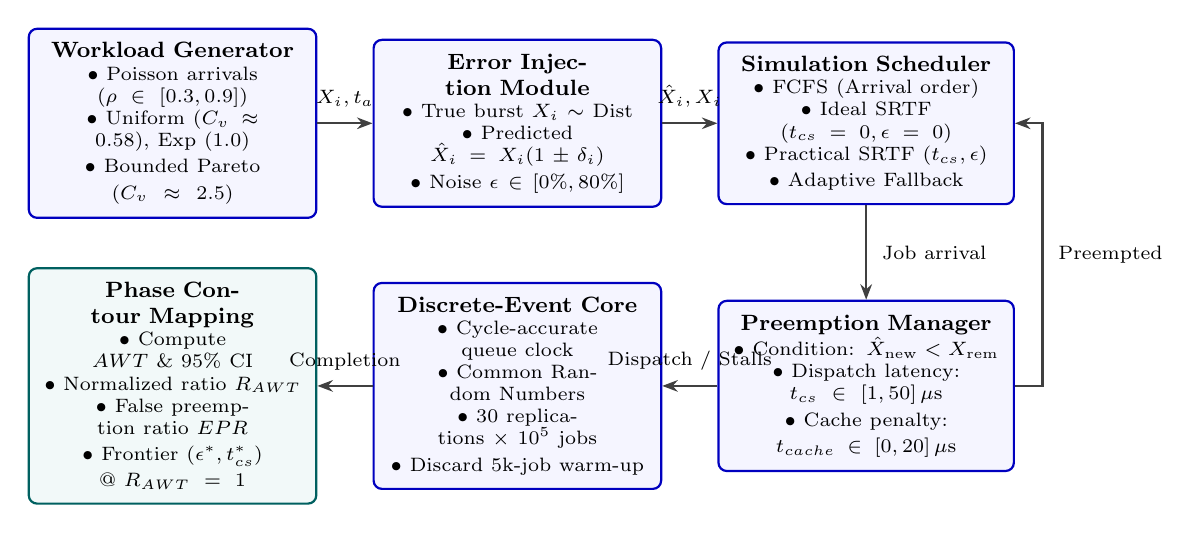
\begin{tikzpicture}[
    >=Stealth,
    node distance=1.1cm and 0.7cm,
    block/.style={rectangle, draw=blue!75!black, fill=blue!4, rounded corners=3pt, thick, align=center, font=\footnotesize, inner sep=5pt, minimum height=1.3cm},
    param/.style={rectangle, draw=gray!60, fill=gray!6, dashed, rounded corners=2pt, font=\scriptsize, align=center, inner sep=3pt},
    outblock/.style={rectangle, draw=teal!75!black, fill=teal!5, rounded corners=3pt, thick, align=center, font=\footnotesize, inner sep=5pt, minimum height=1.3cm},
    line/.style={draw=black!75, -{Stealth[scale=0.85]}, thick}
]

% Row 1: Generation & Noise & Scheduler
\node[block, text width=3.3cm] (gen) {\textbf{Workload Generator}\\ \scriptsize $\bullet$ Poisson arrivals ($\rho \in [0.3, 0.9]$)\\ $\bullet$ Uniform ($C_v \approx 0.58$), Exp ($1.0$)\\ $\bullet$ Bounded Pareto ($C_v \approx 2.5$)};

\node[block, text width=3.3cm, right=0.7cm of gen] (noise) {\textbf{Error Injection Module}\\ \scriptsize $\bullet$ True burst $X_i \sim \text{Dist}$\\ $\bullet$ Predicted $\hat{X}_i = X_i (1 \pm \delta_i)$\\ $\bullet$ Noise $\epsilon \in [0\%, 80\%]$};

\node[block, text width=3.4cm, right=0.7cm of noise] (sched) {\textbf{Simulation Scheduler}\\ \scriptsize $\bullet$ FCFS (Arrival order)\\ $\bullet$ Ideal SRTF ($t_{cs}=0, \epsilon=0$)\\ $\bullet$ Practical SRTF ($t_{cs}, \epsilon$)\\ $\bullet$ Adaptive Fallback};

\draw[line] (gen) -- node[above=2pt, font=\scriptsize] {$X_i, t_a$} (noise);
\draw[line] (noise) -- node[above=2pt, font=\scriptsize] {$\hat{X}_i, X_i$} (sched);

% Row 2: Preemption, CPU, Metrics (placed below top row with clean clearance)
\node[block, text width=3.4cm, below=1.2cm of sched] (preempt) {\textbf{Preemption Manager}\\ \scriptsize $\bullet$ Condition: $\hat{X}_{\text{new}} < X_{\text{rem}}$\\ $\bullet$ Dispatch latency: $t_{cs} \in [1, 50]\,\mu\text{s}$\\ $\bullet$ Cache penalty: $t_{cache} \in [0, 20]\,\mu\text{s}$};

\node[block, text width=3.3cm, left=0.7cm of preempt] (cpu) {\textbf{Discrete-Event Core}\\ \scriptsize $\bullet$ Cycle-accurate queue clock\\ $\bullet$ Common Random Numbers\\ $\bullet$ 30 replications $\times$ $10^5$ jobs\\ $\bullet$ Discard 5k-job warm-up};

\node[outblock, text width=3.3cm, left=0.7cm of cpu] (metrics) {\textbf{Phase Contour Mapping}\\ \scriptsize $\bullet$ Compute $AWT$ \& $95\%$ CI\\ $\bullet$ Normalized ratio $R_{AWT}$\\ $\bullet$ False preemption ratio $EPR$\\ $\bullet$ Frontier $(\epsilon^*, t_{cs}^*)$ @ $R_{AWT}=1$};

\draw[line] (sched) -- node[right=2pt, font=\scriptsize] {Job arrival} (preempt);
\draw[line] (preempt) -- node[above=2pt, font=\scriptsize] {Dispatch / Stalls} (cpu);
\draw[line] (cpu) -- node[above=2pt, font=\scriptsize] {Completion} (metrics);

% Feedback loop for preempted job returning to queue
\draw[line] (preempt.east) -- ++(0.35,0) |- node[near start, right=2pt, font=\scriptsize] {Preempted} ($(sched.east)+(0,0)$);

\end{tikzpicture}
\caption{Trace-driven discrete-event simulation pipeline: from workload generation and error injection to hardware preemption modeling and multi-variable crossover boundary extraction.}\label{fig:deliverable3_pipeline}
\end{figure}

% ============================================================================================
% PAGE 10: STAGE 4 (TASK E & DELIVERABLE 4 RISK MATRIX)
% ============================================================================================
\newpage
{\centering\fontsize{13}{16}\selectfont\textbf{Stage 4 --- Identify Research Risks and Limitations}\par}
\vspace{0.3em}

\topicTitle{Task E: Feasibility and Limitations}

Translating theoretical scheduling questions into an empirical simulation study exposes several methodological and systems-level challenges. Uncontrolled experimental factors, oversimplified architectural assumptions, or sampling noise could bias performance boundaries or compromise reproducibility. Below, we identify five distinct technical challenges spanning hardware fidelity, statistical inference, workload representativeness, error structure, and architectural scope, pairing each with a concrete, realistic mitigation strategy.

\vspace{0.35em}
\topicTitle{Deliverable 4: Research Feasibility, Potential Challenges, and Mitigation Strategies Table}

Table~\ref{tab:deliverable4_risks} presents the identified technical challenges, their operational impact on experimental validity, and our concrete mitigation strategies.

\vspace{0.2em}
{\footnotesize
\setlength{\tabcolsep}{3.5pt}
\renewcommand{\arraystretch}{0.94}
{\centering
\begin{tabular}{|>{\raggedright\arraybackslash}p{2.6cm}|>{\raggedright\arraybackslash}p{2.3cm}|>{\raggedright\arraybackslash}p{4.7cm}|>{\raggedright\arraybackslash}p{6.4cm}|}
    \hline
    \textbf{Potential Challenge} & \textbf{Risk Level \& Category} & \textbf{Operational Impact on Proposed Research} & \textbf{Realistic Mitigation Strategy} \\
    \hline
    
    \textbf{1. Cache Perturbation \& Memory Hierarchy Fidelity} & 
    Moderate \newline \textit{(Architectural Validity)} & 
    Treating cache warm-up delay as a single static constant ($t_{cache}$) risks oversimplifying dynamic working-set eviction, cache line bouncing, and TLB reload penalties on physical CPUs. & 
    Calibrate $t_{cache}$ bounds using hardware Performance Monitoring Unit (PMU) counters on real cores running Linux \texttt{perf} (tracking L1/LLC misses), and sweep $t_{cache} \in [0, 20]\,\mu\text{s}$ to establish parametric sensitivity bounds. \\
    \hline

    \textbf{2. Statistical Uncertainty Near the Crossover Boundary} & 
    High \newline \textit{(Measurement \& Statistics)} & 
    As the waiting-time ratio approaches unity ($R_{AWT} \to 1.0$), stochastic variance across replication seeds can introduce jitter and blur the contour line $(\epsilon^*, t_{cs}^*)$. & 
    Enforce Common Random Numbers (CRN) across all algorithms so that comparisons evaluate strictly paired sample paths. Execute 30 independent replications per grid point ($10^5$ jobs each) and apply cubic spline interpolation with 95\% confidence intervals. \\
    \hline

    \textbf{3. Synthetic Workload Skew \& Trace Bias} & 
    Moderate \newline \textit{(External Validity)} & 
    Idealized mathematical distributions (Uniform, Exponential, Pareto) may lack temporal autocorrelation, burstiness bursts, and phase shifts found in production server workloads. & 
    Complement synthetic models with empirical trace replay from public cloud/supercomputing repositories (e.g., Google Cluster and Parallel Workloads traces), verifying that synthetic crossover trends hold under realistic traffic. \\
    \hline

    \textbf{4. Temporal Autocorrelation in Prediction Errors} & 
    Moderate \newline \textit{(Modeling Fidelity)} & 
    Assuming independent, identically distributed (i.i.d.) Gaussian error may underestimate thrashing if real runtime predictors (e.g., EWMA) suffer from bursty, auto-correlated estimation lag. & 
    Implement dual error-injection models: standard i.i.d.\ noise and a first-order autoregressive AR(1) error model ($\rho_{err} \in [0.2, 0.8]$), explicitly evaluating how clustered estimation errors degrade SRTF stability. \\
    \hline

    \textbf{5. Single-Core Queuing vs.\ Multi-Core Generalization} & 
    Low to Moderate \newline \textit{(Generalizability)} & 
    A single-core uniprocessor queue abstracts away multi-core phenomena such as NUMA locality, inter-core task migration overhead, and distributed run-queue lock contention. & 
    Formally define the single-core queue as the fundamental theoretical baseline (consistent with classical $M/G/1$ scheduling theory), and architect the simulation framework with modular multi-queue hooks for future SMP scaling. \\
    \hline
\end{tabular}\par
}
\vspace{-0.6em}
\captionof{table}{Research Feasibility, Potential Challenges, and Realistic Mitigation Strategies Matrix}\label{tab:deliverable4_risks}
}

% ============================================================================================
% PAGE 11: STAGE 5 (TASK F & DELIVERABLE 5: MINI RESEARCH PROPOSAL - PART 1)
% ============================================================================================
\newpage
{\centering\fontsize{13}{16}\selectfont\textbf{Stage 5 --- Write a Mini Research Proposal}\par}
\vspace{0.3em}

\topicTitle{Task F: Mini Research Proposal}

We synthesize our refined research question, objectives, hypotheses, methodology, and risk mitigations into a self-contained mini research proposal of 500--700 words, structured across the seven required components and citing established academic literature [1--6].

\vspace{0.35em}
\topicTitle{Deliverable 5: Structured Mini Research Proposal}

\begin{enumerate}[label=\textbf{\arabic*.}, leftmargin=1.4em, itemsep=0.45em, parsep=0pt]

    \item \textbf{Proposed Research Title:} \\
    Quantifying the Multi-Variable Crossover Boundary of Shortest Remaining Time First Scheduling Under Estimation Noise and Context-Switch Latency.

    \item \textbf{Background and Motivation:} \\
    Modern CPU scheduling balances responsiveness against dispatcher switching overhead [1, 5]. Classical queuing theory establishes that Shortest Remaining Time First (SRTF) minimizes average waiting time in uniprocessor queues [6]. However, this optimality strictly assumes perfect advance knowledge of burst durations and zero-cost preemption [5, 6]. Foundational studies show that size-based scheduling resists prediction errors in heavy-tailed workloads, where coarse sorting prevents long tasks from blocking short jobs [3, 4]. Wierman and Nuyens proved this analytically under bounded noise, but assumed costless preemption ($t_{cs} = 0$) [4]. In physical systems, estimation errors cause false preemptions, incurring register swaps, TLB flushes, and cache misses [5]. In low-variance workloads, size-based prioritization yields minimal queueing gains, leaving systems vulnerable to thrashing where First-Come-First-Served (FCFS) may achieve superior efficiency [1, 2].

    \item \textbf{Research Problem and Identified Research Gap:} \\
    While size-based scheduling withstands estimation noise under costless preemption in heavy-tailed traffic [3, 4], the combined impact of prediction error ($\epsilon$) and physical context-switch latency ($t_{cs}$) remains unquantified. Specifically, published literature lacks an empirical mapping of the multi-variable crossover boundary $(\epsilon^*, t_{cs}^*)$ where SRTF's waiting-time advantage degrades or reverses ($AWT_{\text{SRTF}} \ge AWT_{\text{FCFS}}$) in non-heavy-tailed workloads (Uniform and Exponential), where preemption costs cannot be masked by workload skew.

    \item \textbf{Research Objectives:} \\
    This investigation pursues three measurable objectives:
    \begin{enumerate}[label=(\alph*), leftmargin=1.2em, itemsep=0.15em]
        \item Quantify false preemption rates and cumulative CPU stalls across error $\epsilon \in [0\%, 80\%]$ and latency $t_{cs} \in [1, 50]\,\mu\text{s}$.
        \item Map the parametric crossover boundary $(\epsilon^*, t_{cs}^*)$ across traffic loads ($\rho \in \{0.3$, $0.5$, $0.7$, $0.9\}$) delineating SRTF-superior and FCFS-superior regimes.
        \item Evaluate boundary sensitivity across workload coefficient of variation ($C_v \in [0.58, 2.5]$) and benchmark an adaptive fallback heuristic that reverts to FCFS when noise exceeds threshold.
    \end{enumerate}

    \item \textbf{Proposed Methodology:} \\
    To eliminate OS daemon jitter and dynamic frequency scaling, we deploy a trace-driven, discrete-event simulation harness. Workloads comprise synthetic distributions (Uniform, Exponential, Bounded Pareto) and empirical supercomputing traces with identical mean execution time ($E[X] = 10$\,ms) under Poisson arrivals. We compare four policies: FCFS, Ideal SRTF ($\epsilon=0, t_{cs}=0$), Practical SRTF (with noise $\epsilon$, context latency $t_{cs}$, and cache delay $t_{cache}$), and Adaptive Fallback. Common Random Numbers across 30 independent replications of 100,000 jobs ensure paired comparisons. A 5,000-job warm-up is discarded, and metrics ($AWT$, $R_{AWT}$, $EPR$) are reported with 95\% confidence intervals.

\end{enumerate}

% ============================================================================================
% PAGE 12: STAGE 5 (TASK F & DELIVERABLE 5: PROPOSAL PART 2 & SYSTEMS DISCUSSION)
% ============================================================================================
\newpage
\begin{enumerate}[label=\textbf{\arabic*.}, leftmargin=1.4em, itemsep=0.45em, parsep=0pt, resume]

    \item \textbf{Expected Contribution:} \\
    Our investigation expects to deliver three distinct contributions that contrast with established theory:
    \begin{enumerate}[label=(\roman*), leftmargin=1.2em, itemsep=0.2em]
        \item An empirical phase map providing the first characterization of the $(\epsilon^*, t_{cs}^*)$ crossover contour, proving that SRTF superiority is non-universal when preemption penalties are included.
        \item A quantitative model showing that workload variance ($C_v$) acts as a protective buffer, such that low-variance workloads contract SRTF's dominance zone by $>50\%$.
        \item An empirically grounded adaptive fallback heuristic offering OS scheduler designers concrete switching thresholds to prevent preemption thrashing.
    \end{enumerate}

    \item \textbf{Limitations and Future Scope:} \\
    The primary limitation is the uniprocessor queue abstraction, which excludes multi-core cache coherence and inter-core migration delays. Future extensions will investigate Symmetric Multiprocessing (SMP) architectures, asymmetric CPU topologies (big.LITTLE), and online machine-learning burst predictors.

\end{enumerate}



\vspace{0.6em}
\topicTitle{Operating System Implementation Perspectives and Practical Relevance}

The findings of this proposed research have direct engineering implications for next-generation operating system kernel schedulers and container runtimes:
\begin{enumerate}[label=\textbf{\alph*.}, leftmargin=1.4em, itemsep=0.35em, parsep=0pt]
    \item \textbf{Kernel Scheduler Design in Linux eBPF (\texttt{sched\_ext}):} With the recent integration of extensible scheduler architectures in Linux via \texttt{sched\_ext}, systems programmers can dynamically implement user-defined scheduling policies. Our mapped crossover contour $(\epsilon^*, t_{cs}^*)$ provides concrete mathematical guardrails: instead of running unconditional shortest-job prioritization, the scheduler can continuously monitor burst prediction variance and automatically revert to arrival-ordered dispatching when thrashing is imminent.
    \item \textbf{Containerized Microservices and Serverless Computing:} In cloud native platforms (Kubernetes and AWS Lambda), execution bursts for RPC request handlers exhibit moderate variance ($C_v \approx 0.8$--$1.2$) and sub-millisecond durations. In these microsecond-scale environments, context switching and cold-cache penalties consume up to 25\% of total execution time. Delineating preemption crossover thresholds prevents catastrophic performance collapse under noisy burst estimates.
    \item \textbf{Architectural Co-Design with Hardware Performance Counters:} Operating systems can leverage hardware Performance Monitoring Units (PMUs) to dynamically sample Last Level Cache (LLC) misses. If cache reload latency spikes during preemption-heavy phases, the kernel can adaptively raise preemption hysteresis thresholds, thereby preserving CPU throughput.
\end{enumerate}

% ============================================================================================
% PAGE 13: STAGE 6 (STUDENT 1: GAURAV ACHARYA)
% ============================================================================================
\newpage
{\centering\fontsize{13}{16}\selectfont\textbf{Stage 6 --- Individual Critical Reflection}\par}
\vspace{0.35em}

\topicTitle{Task G \& Deliverable 6: Individual Critical Reflection}

Each group member independently reflects on the technical formulation, methodological validity, risk criteria, and epistemological evolution of this proposed research.

\vspace{0.4em}
\topicTitle{Student 1: Gaurav Acharya (MT26MCS024)}

\begin{enumerate}[label=\textbf{\arabic*.}, leftmargin=1.4em, itemsep=0.6em, parsep=0pt]
    \item \textbf{What is the most difficult aspect of converting your research gap into a feasible research study?} \\
    The most difficult aspect was translating abstract hardware overheads---specifically cache warm-up and TLB invalidation---into tractable simulation variables without sacrificing architectural realism. While theoretical gap formulation easily identifies context switching as a missing parameter, physical CPU penalties vary widely with working-set sizes and memory bus contention. Calibrating realistic latency bounds $t_{cache} \in [0, 20]\,\mu\text{s}$ that reflect physical execution without simulating the entire cycle-level microarchitecture was our steepest design hurdle.

    \item \textbf{Which assumption in your proposed methodology is most likely to affect the validity of your results?} \\
    The assumption most likely to affect validity is modeling the cache reload delay ($t_{cache}$) as an independent additive latency. In real operating systems, cache degradation depends heavily on cache footprint overlap and inter-process spatial locality. If a preempting task has a small working set, cache line pollution is minimal; if large, penalties are catastrophic. Assuming fixed or independently distributed delays simplifies discrete-event queuing, but risks either understating or overstating preemption severity.

    \item \textbf{What evidence would make you reconsider or abandon your proposed research question?} \\
    I would abandon the research question if preliminary simulation showed that even with extreme prediction errors ($\epsilon > 60\%$) and high switching latencies ($t_{cs} = 50\,\mu\text{s}$), SRTF maintained lower average waiting times than FCFS across all tested distributions. Such evidence would prove that coarse prioritization remains overwhelmingly dominant regardless of hardware overhead, rendering the proposed crossover boundary practically nonexistent and eliminating the empirical necessity of an adaptive fallback scheduler.

    \item \textbf{How has your understanding of research novelty changed from Practical 5 to Practical 9?} \\
    In Practical 5, I assumed novelty meant inventing an entirely new scheduling algorithm from scratch. By Practical 9, I realized that genuine novelty often lies in rigorous boundary critique: identifying unstated, fragile assumptions in classical theory and quantifying where established optimality claims collapse. Demonstrating that textbook algorithms fail under realistic physical overheads and mapping the parameter crossover frontier provides substantial, defensible scientific contribution without proposing complex, untested algorithms.
\end{enumerate}

% ============================================================================================
% PAGE 14: STAGE 6 (STUDENT 2: SANDEEP & AI DISCLOSURE)
% ============================================================================================
\newpage
\topicTitle{Student 2: Sandeep (MT26MCS032)}

\begin{enumerate}[label=\textbf{\arabic*.}, leftmargin=1.4em, itemsep=0.6em, parsep=0pt]
    \item \textbf{What is the most difficult aspect of converting your research gap into a feasible research study?} \\
    The greatest challenge was designing an evaluation framework that isolates the crossover boundary $(\epsilon^*, t_{cs}^*)$ from confounding queueing dynamics. Near $R_{AWT} \approx 1.0$, random seed variance easily creates statistical noise that obscures the true contour. Balancing computational feasibility across thousands of parameter combinations while executing sufficient replications ($30 \times 10^5$ jobs) and warm-up discards to guarantee tight 95\% confidence intervals demanded careful simulation engineering and variance-reduction planning. 

    \item \textbf{Which assumption in your proposed methodology is most likely to affect the validity of your results?} \\
    Assuming a uniprocessor system with independent Poisson arrivals represents the greatest threat to validity. Modern cloud compute engines operate on multicore symmetric multiprocessing (SMP) nodes with thread affinity, work-stealing schedulers, and NUMA memory nodes. While single-core queues serve as the necessary theoretical baseline for classical scheduling analysis, multicore load-balancing could mitigate preemption delays by migrating preempted threads to idle cores, potentially shifting the empirical crossover boundary rightward.

    \item \textbf{What evidence would make you reconsider or abandon your proposed research question?} \\
    I would reconsider the question if trace replays of real enterprise workloads revealed that burst prediction accuracy in modern runtimes consistently achieves errors below 5\% ($\epsilon < 5\%$). At such negligible noise levels, false preemptions rarely happen, meaning SRTF would never approach the crossover threshold under realistic context-switch latencies ($t_{cs} \le 15\,\mu\text{s}$). The research question would lose practical relevance for production operating systems.

    \item \textbf{How has your understanding of research novelty changed from Practical 5 to Practical 9?} \\
    My perspective shifted from broad, ambitious declarations toward precise, defendable parameter boundaries. In Practical 5, our group proposed a sweeping claim that SRTF is impractical for operating systems. Through systematic literature critique and gap formulation in Practicals 7--9, I learned that research becomes novel and defensible only when narrowed: isolating specific workload distributions (low-variance non-heavy-tailed) and explicitly parameterizing physical context-switch and cache costs that existing models ignored.
\end{enumerate}

\vspace{0.8em}
\noindent\rule{\linewidth}{0.4pt}
\vspace{0.2em}
\topicTitle{Generative AI Assistance Disclosure}
{\footnotesize \noindent
In compliance with the course submission guidelines for CSP529 (Technical Writing \& Publishing), we disclose that generative AI (LLM assistance) was utilized during the preparation of this practical report. Specifically, AI tools were used for LaTeX syntax verification, structural formatting of tabular matrices, drafting block diagram TikZ specifications, and proofreading prose for grammatical clarity and word-count compliance. All research problem definitions, gap analyses, mathematical hypothesis formulations, methodology parameters, critical reflections, and academic citations were independently conceived, verified against original literature, and validated by the student authors. No experimental data or citations were fabricated.
\par}

% ============================================================================================
% PAGE 15: ABBREVIATIONS, NOTATIONS & ACADEMIC REFERENCES
% ============================================================================================
\newpage
\topicTitle{List of Abbreviations and Mathematical Notation Matrix}
{\footnotesize
\setlength{\tabcolsep}{4pt}
\renewcommand{\arraystretch}{0.91}
\noindent
\begin{tabular}{@{}p{1.4cm} p{6.3cm} p{1.4cm} p{6.3cm}@{}}
\toprule
\textbf{Notation} & \textbf{Operational Definition / Unit} & \textbf{Notation} & \textbf{Operational Definition / Unit} \\
\midrule
\textbf{AWT} & Average Waiting Time (milliseconds) & \textbf{PMU} & Performance Monitoring Unit \\
\textbf{ATT} & Average Turnaround Time (milliseconds) & \textbf{SMP} & Symmetric Multiprocessing \\
\textbf{CPU} & Central Processing Unit & \textbf{SRTF} & Shortest Remaining Time First \\
\textbf{CRN} & Common Random Numbers (Variance reduction) & \textbf{SRPT} & Shortest Remaining Processing Time \\
\textbf{DES} & Discrete-Event Simulation & \textbf{TLB} & Translation Lookaside Buffer \\
\textbf{EPR} & Erroneous Preemption Ratio ($N_{\text{err}}/N_{\text{preempt}}$) & \textbf{WSS} & Working Set Size of process (Kilobytes) \\
\textbf{FCFS} & First-Come-First-Served & $\boldsymbol{C_v}$ & Coefficient of Variation ($\sigma / \mu$, dimensionless) \\
\textbf{LLC} & Last Level Cache (CPU memory hierarchy) & $\boldsymbol{\rho}$ & System Traffic Intensity / CPU Load ($\lambda E[X]$) \\
\textbf{NUMA} & Non-Uniform Memory Access & $\boldsymbol{t_{cs}}$ & Hardware Context-Switch Latency ($\mu\text{s}$) \\
\textbf{EWMA} & Exponentially Weighted Moving Average & $\boldsymbol{t_{cache}}$ & Cache Warm-Up Invalidation Delay ($\mu\text{s}$) \\
\textbf{AR(1)} & First-Order Autoregressive Error Model & $\boldsymbol{\epsilon}$ & Relative Burst Prediction Error ($\%$) \\
$\boldsymbol{R_{AWT}}$ & Normalized Waiting Ratio ($AWT_{\text{SRTF}}/AWT_{\text{FCFS}}$) & $\boldsymbol{(\epsilon^*, t_{cs}^*)}$ & Crossover Boundary Contour at $R_{AWT} = 1.0$ \\
\bottomrule
\end{tabular}
}

\vspace{0.6em}
\begin{thebibliography}{9}
\footnotesize
\setlength{\itemsep}{-0.45em}
\setlength{\parsep}{0pt}
\bibitem{reddy2017}
K.~V.~S.~Reddy, ``Comparative analysis of CPU scheduling algorithms for performance efficiency,'' \textit{IJCA}, vol.~168, no.~5, pp.~26--31, 2017.

\bibitem{samanta2020}
P.~Samanta and P.~Biswas, ``Comparative analysis of different CPU scheduling algorithms with respect to average waiting time and average turnaround time,'' \textit{IJARCS}, vol.~11, no.~3, pp.~102--107, 2020.

\bibitem{lu2004}
D.~Lu, H.~Sheng, and P.~A.~Dinda, ``Size-based scheduling policies with inaccurate scheduling information,'' in \textit{Proc. 12th IEEE MASCOTS}, 2004, pp.~31--38.

\bibitem{wierman2008}
A.~Wierman and M.~Nuyens, ``Scheduling despite inexact job-size information,'' \textit{ACM SIGMETRICS PER}, vol.~36, no.~1, pp.~25--36, 2008.

\bibitem{silberschatz2018}
A.~Silberschatz, P.~B.~Galvin, and G.~Gagne, \textit{Operating System Concepts}, 10th~ed.\ Hoboken, NJ, USA: Wiley, 2018.

\bibitem{harchol2013}
M.~Harchol-Balter, \textit{Performance Modeling and Design of Computer Systems: Queueing Theory in Action}. Cambridge, UK: Cambridge University Press, 2013.

\end{thebibliography}

\end{document}
